%%%%%%%%%%%%%%%%%%%%%%%%%%%%%%%%%%%%%%%%%
% Arsclassica Article
% LaTeX Template
% Version 1.1 (1/8/17)
%
% This template has been downloaded from:
% http://www.LaTeXTemplates.com
%
% Original author:
% Lorenzo Pantieri (http://www.lorenzopantieri.net) with extensive modifications by:
% Vel (vel@latextemplates.com)
%
% License:
% CC BY-NC-SA 3.0 (http://creativecommons.org/licenses/by-nc-sa/3.0/)
%
%%%%%%%%%%%%%%%%%%%%%%%%%%%%%%%%%%%%%%%%%

%----------------------------------------------------------------------------------------
%	PACKAGES AND OTHER DOCUMENT CONFIGURATIONS
%----------------------------------------------------------------------------------------

\documentclass[
10pt, % Main document font size
a4paper, % Paper type, use 'letterpaper' for US Letter paper
oneside, % One page layout (no page indentation)
DIV=16,
parskip=full,
%twoside, % Two page layout (page indentation for binding and different headers)
headinclude,footinclude % Extra spacing for the header and footer
]{scrartcl}

%%%%%%%%%%%%%%%%%%%%%%%%%%%%%%%%%%%%%%%%%
% Arsclassica Article
% Structure Specification File
%
% This file has been downloaded from:
% http://www.LaTeXTemplates.com
%
% Original author:
% Lorenzo Pantieri (http://www.lorenzopantieri.net) with extensive modifications by:
% Vel (vel@latextemplates.com)
%
% License:
% CC BY-NC-SA 3.0 (http://creativecommons.org/licenses/by-nc-sa/3.0/)
%
%%%%%%%%%%%%%%%%%%%%%%%%%%%%%%%%%%%%%%%%%

%----------------------------------------------------------------------------------------
%	REQUIRED PACKAGES
%----------------------------------------------------------------------------------------

\usepackage[
nochapters, % Turn off chapters since this is an article        
beramono, % Use the Bera Mono font for monospaced text (\texttt)
eulermath,% Use the Euler font for mathematics
pdfspacing, % Makes use of pdftex’ letter spacing capabilities via the microtype package
dottedtoc % Dotted lines leading to the page numbers in the table of contents
]{classicthesis} % The layout is based on the Classic Thesis style

\usepackage{arsclassica} % Modifies the Classic Thesis package

\usepackage[T1]{fontenc} % Use 8-bit encoding that has 256 glyphs

\usepackage[utf8]{inputenc} % Required for including letters with accents

\usepackage{graphicx} % Required for including images
\graphicspath{{Figures/}} % Set the default folder for images

\usepackage{enumitem} % Required for manipulating the whitespace between and within lists

\usepackage{lipsum} % Used for inserting dummy 'Lorem ipsum' text into the template

\usepackage{subfig} % Required for creating figures with multiple parts (subfigures)

\usepackage{amsmath,amssymb,amsthm} % For including math equations, theorems, symbols, etc

\usepackage{varioref} % More descriptive referencing

%----------------------------------------------------------------------------------------
%	THEOREM STYLES
%---------------------------------------------------------------------------------------

\theoremstyle{definition} % Define theorem styles here based on the definition style (used for definitions and examples)
\newtheorem{definition}{Definition}

\theoremstyle{plain} % Define theorem styles here based on the plain style (used for theorems, lemmas, propositions)
\newtheorem{theorem}{Theorem}

\theoremstyle{remark} % Define theorem styles here based on the remark style (used for remarks and notes)

%----------------------------------------------------------------------------------------
%	HYPERLINKS
%---------------------------------------------------------------------------------------

\hypersetup{
%draft, % Uncomment to remove all links (useful for printing in black and white)
colorlinks=true, breaklinks=true, bookmarks=true,bookmarksnumbered,
urlcolor=webbrown, linkcolor=RoyalBlue, citecolor=webgreen, % Link colors
pdftitle={}, % PDF title
pdfauthor={\textcopyright}, % PDF Author
pdfsubject={}, % PDF Subject
pdfkeywords={}, % PDF Keywords
pdfcreator={pdfLaTeX}, % PDF Creator
pdfproducer={LaTeX with hyperref and ClassicThesis} % PDF producer
}

%----------------------------------------------------------------------------------------
% EXTRAS
%----------------------------------------------------------------------------------------

\newcommand{\bluetext}{\textcolor{blue}}  % colored text for review
 % Include the structure.tex file which specified the document structure and layout

\hyphenation{Fortran hy-phen-ation} % Specify custom hyphenation points in words with dashes where you would like hyphenation to occur, or alternatively, don't put any dashes in a word to stop hyphenation altogether


%----------------------------------------------------------------------------------------
%	TITLE AND AUTHOR(S)
%----------------------------------------------------------------------------------------

\title{\normalfont\spacedallcaps{Measuring death rates in New Zealand}} % The article title

\subtitle{NOT OFFICIAL STATISTICS. This is a living technical note detailing the technical aspects of the EXPERIMENTAL measures in presented in this repository.} 

\author{\spacedlowsmallcaps{Statistics New Zealand* }} % The article author(s) - author affiliations need to be specified in the AUTHOR AFFILIATIONS block

\date{} % An optional date to appear under the author(s)

%----------------------------------------------------------------------------------------

\begin{document}


%----------------------------------------------------------------------------------------
%	HEADERS
%----------------------------------------------------------------------------------------

\renewcommand{\sectionmark}[1]{\markright{\spacedlowsmallcaps{#1}}} % The header for all pages (oneside) or for even pages (twoside)
%\renewcommand{\subsectionmark}[1]{\markright{\thesubsection~#1}} % Uncomment when using the twoside option - this modifies the header on odd pages
\lehead{\mbox{\llap{\small\thepage\kern1em\color{halfgray} \vline}\color{halfgray}\hspace{0.5em}\rightmark\hfil}} % The header style

\pagestyle{scrheadings} % Enable the headers specified in this block

%----------------------------------------------------------------------------------------
%	TABLE OF CONTENTS & LISTS OF FIGURES AND TABLES
%----------------------------------------------------------------------------------------

\maketitle % Print the title/author/date block

\setcounter{tocdepth}{2} % Set the depth of the table of contents to show sections and subsections only

\tableofcontents % Print the table of contents

\listoffigures % Print the list of figures

%\listoftables % Print the list of tables

%----------------------------------------------------------------------------------------
%	AUTHOR AFFILIATIONS
%----------------------------------------------------------------------------------------
\begingroup%
\let\thefootnote\relax\footnotetext{* \textit{Authored by Pubudu Senanayake and Lucianne Varn on behalf of Statistics New Zealand}}
\endgroup%
%----------------------------------------------------------------------------------------

\newpage % Start the article content on the second page, remove this if you have a longer abstract that goes onto the second page

%----------------------------------------------------------------------------------------
%	INTRODUCTION
%----------------------------------------------------------------------------------------

%-----------------------------------------------
\section{Introduction}\label{sec:intro}
%-----------------------------------------------

With COVID-19 now widely prevalent in New Zealand, understanding the impacts on the health of the community is critical. Examining the deaths that may be associated with COVID-19 provides a measure of how the country is impacted. However, given the prevalence in the community there are two points to consider:

\begin{itemize}
    \item Some deaths associated with COVID-19 are not correctly attributed to the disease (as has been observed in other jurisdictions);
    \item Some incidental deaths are associated with COVID-19 because of the reporting regime (death within 28 days of testing positive for COVID-19).
\end{itemize}

One of the ways to gain insight into whether COVID-19 is driving a change in mortality is to examine "excess deaths" in the community. This is considered one of the most objective ways of understanding the impact of COVID-19 on the community \cite{Bearny2020}, assuming expectations can be accurately computed. This is particularly so for jurisdictions with large numbers of deaths. 

Typically, \textit{excess deaths} refer to all-cause deaths above deaths expected under normal conditions, derived from observations prior to the period of the event of interest \cite{karlinsky2021tracking}. The main unreliability of these measures emerges in establishing deaths "expected under normal conditions". The measures discussed in this note suffer from this weakness, so they should be used with caution.

In 2022, for the first time since the beginning of the pandemic NZ has had to deal with widespread COVID-19 in the community. Establishing a measure of expected deaths and tracking the deaths across 2022, will provide insight into potential emerging problems where intervention may be needed.


%----------------------------------------------------------------------------------------
%	METHODS
%----------------------------------------------------------------------------------------

%--------------------------------------------------------
\section{Measures of expected deaths}\label{sec:method}
%--------------------------------------------------------

In order to understand how the currently observed deaths are tracking, we must first establish a measure of expected deaths. We will take two approaches, thus establishing two measures of expected deaths:

\begin{enumerate}[noitemsep] % [noitemsep] removes whitespace between the items for a compact look
\item Pre-pandemic death rate averages;
\item Pre-pandemic death rate trends projected into the pandemic years. -- under development
\end{enumerate}

These measures are then compared to the death rates (across different age groups) during the pandemic years. Both of these approaches are used by the Human Mortality Database's Short Term Mortality Fluctuations data series, a series that examines excess deaths across a number of jurisdictions throughout the pandemic \cite{hmd_excess2021}.

Note that these measures are based on death rates instead of counts. It is important to use measures based on death rates when establishing expected deaths, because raw counts can be misleading. In an ageing population (such as New Zealand) raw death counts generally rise, regardless of external conditions. Therefore, simply examining raw counts convolutes an unavoidable factor (ageing population) with factors that can (at least hypothetically) be mitigated (e.g., infectious diseases).

\begin{figure}[htb!]
\centering 
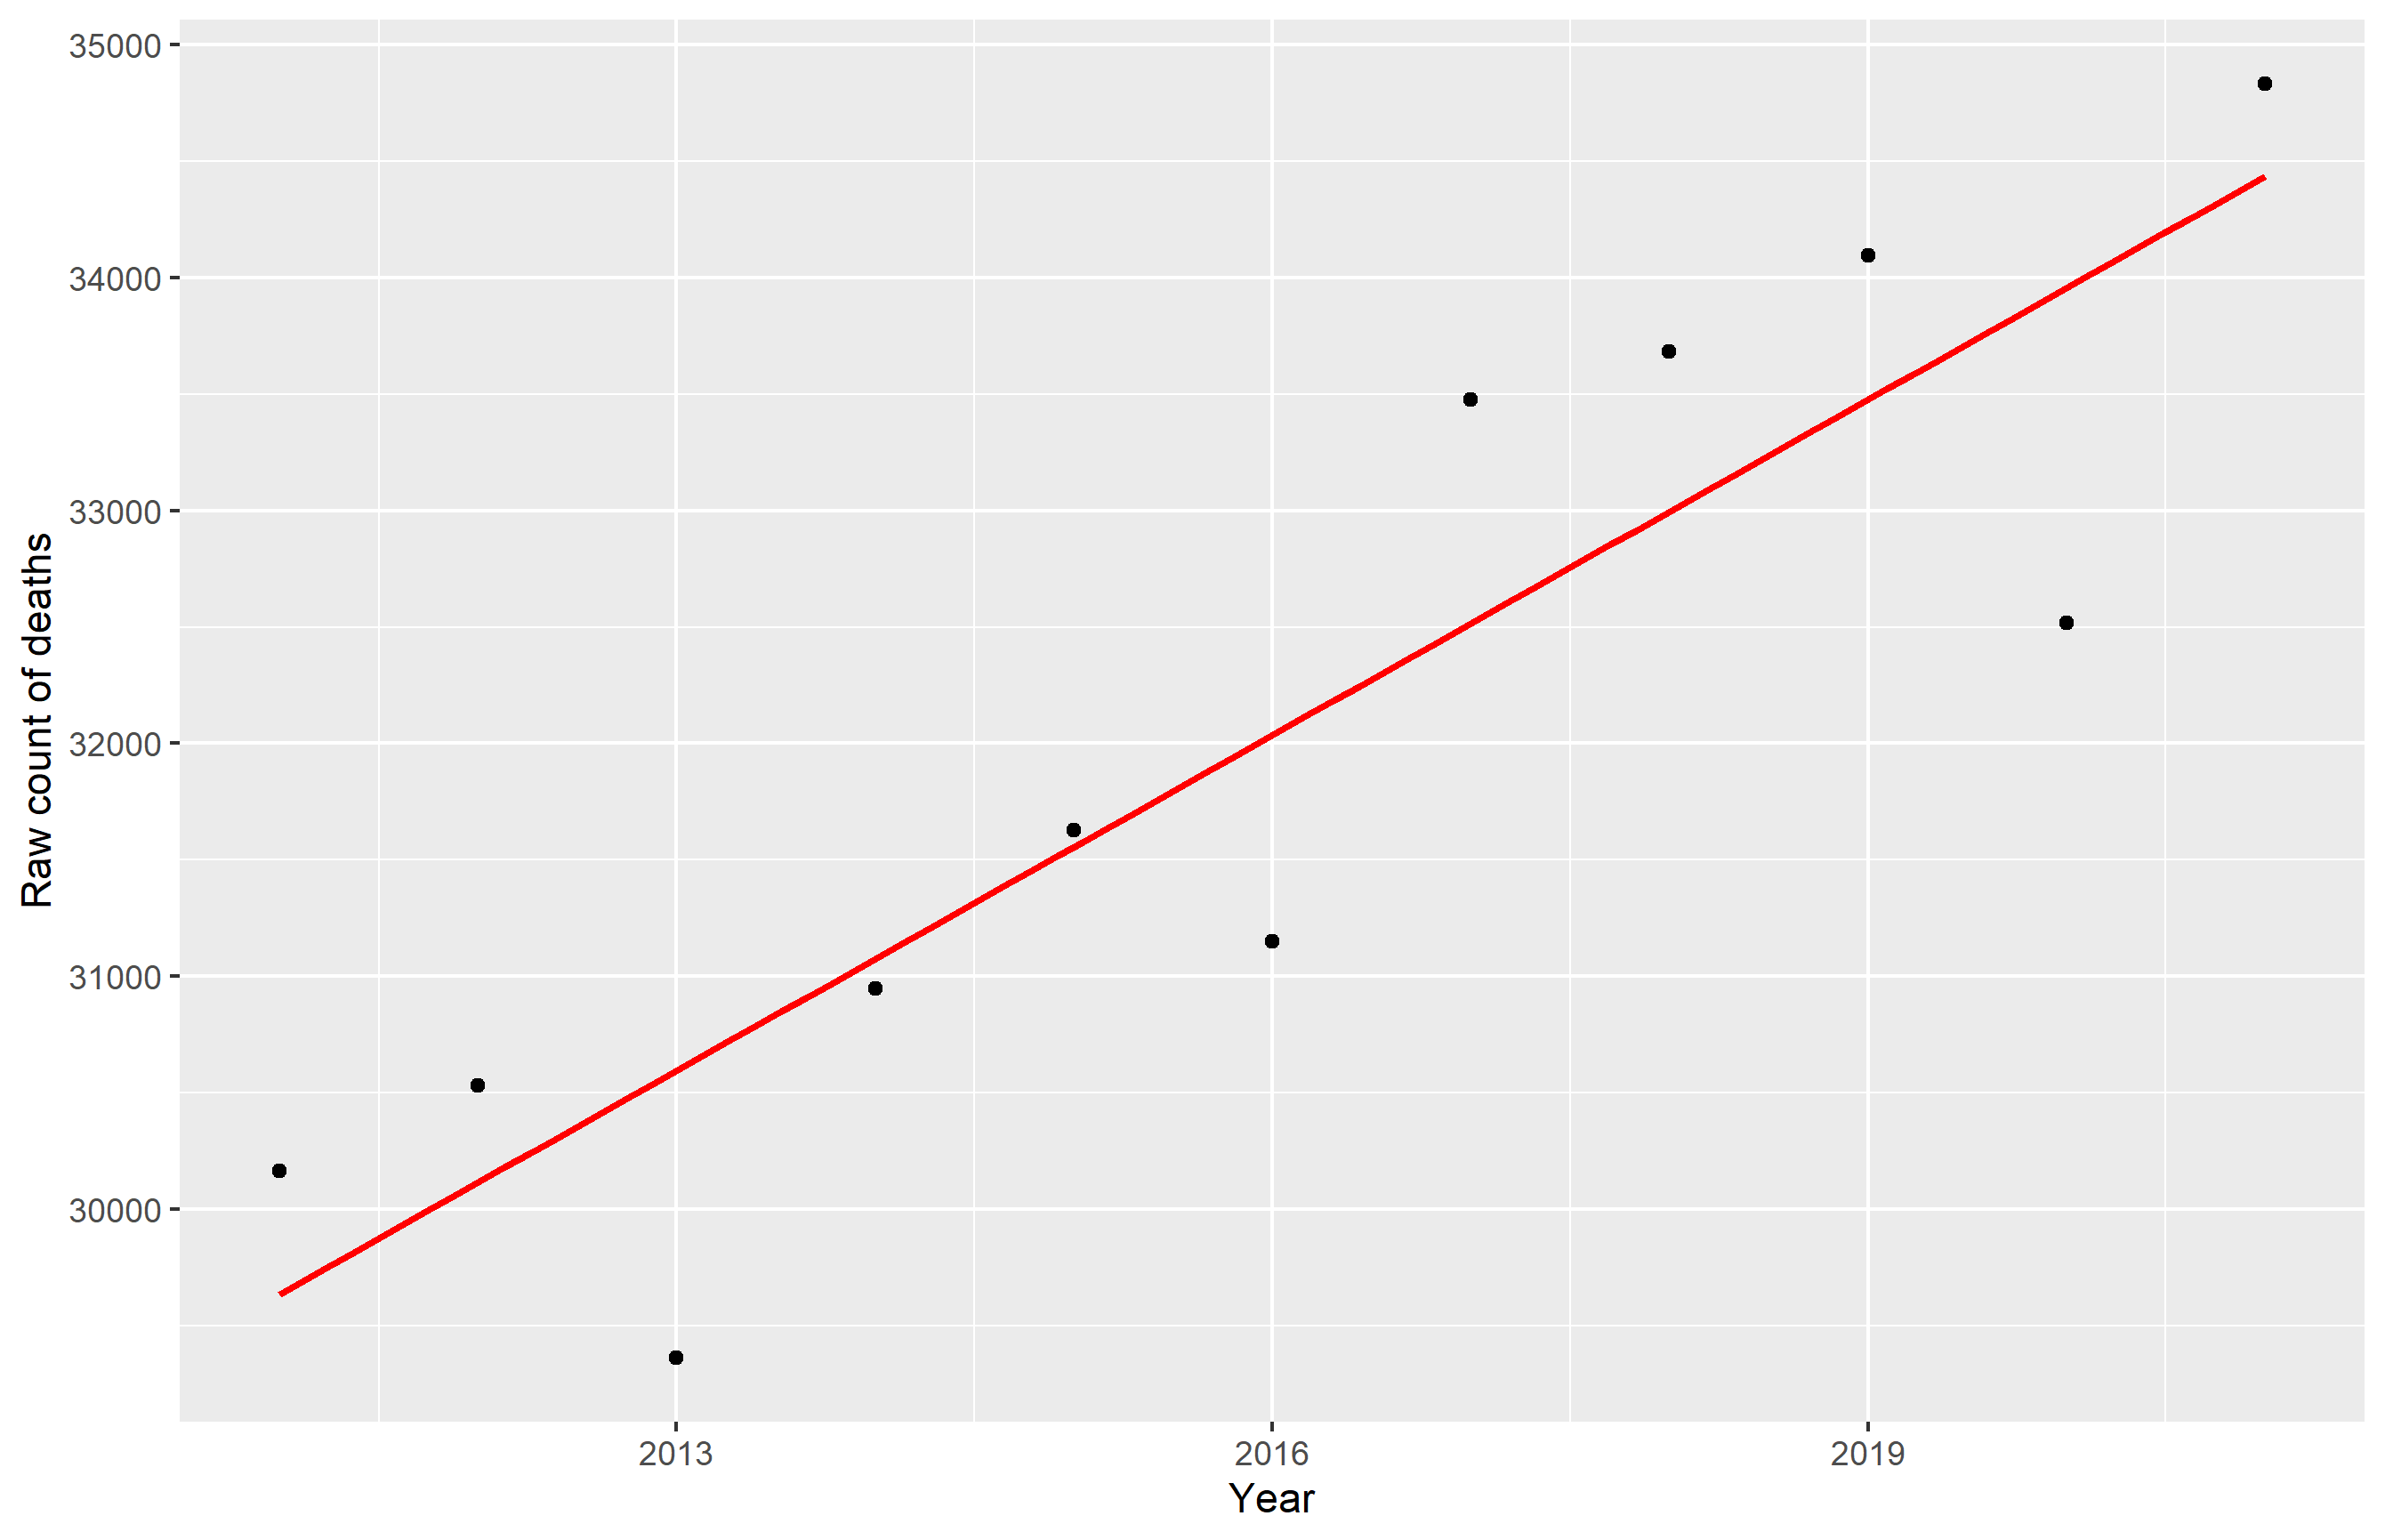
\includegraphics[width = 1.0 \columnwidth]{plots/deaths_over_time} 
\caption[Annual deaths over time]{Annual all-cause deaths from 2011 to 2021. The overall increase in death numbers, driven by New Zealand's ageing population is clear.} 
\label{fig:deaths_time} 
\end{figure}

Figure~\vref{fig:deaths_time} shows how New Zealand death counts track over the years, and the general trend of increasing numbers due to an ageing population is evident when examining the time series. It should be noted however, that given more people are ageing into older age groups, any external factors that increase the baseline mortality within these age groups (e.g., COVID-19 circulating freely in the 80+ population say) will lead to a higher baseline level of death. This cannot be purely ascribed to the ageing of the population.


%--------------------------------------------------------------------
\subsection{Data used for estimating death rates}\label{subsec:data}
%--------------------------------------------------------------------

In this analysis, the deaths during the pandemic years are compared to expected total deaths (crude death rates) and expected deaths by age groups (age-specific death rates) derived from pre-pandemic death counts. 

Two pieces of data are required to construct a time series of these death rates:

\begin{itemize}
    \item Death counts over time periods (e.g., months), for the population groups of interest (e.g., age groups);
    \item Population counts across the same time periods as the death counts, for the population groups of interest.
\end{itemize}

\paragraph{Deaths data} Deaths data are provided by the New Zealand Department of Internal Affairs (DIA). This is a time series of weekly deaths, starting in 2011, and reported with about a two week lag. The weekly death counts are broken down into age groups, specifically, 0 -- 4, 5 -- 29, 30 -- 59, and 5 year age groups from 60 years onwards. Deaths are reported to DIA by date of death, and DIA provides Statistics New Zealand the aggregated weekly death counts derived from these reported deaths.

The deaths time series is a weekly series, ranging from week 1 to week 52 of a year. This allows comparisons of trajectories across the years -- for example, allowing us to compare the effect of different winter seasons. Figure~\vref{fig:deaths_data} shows the observed total weekly deaths across selected years.

\begin{figure}[htb!]
\centering 
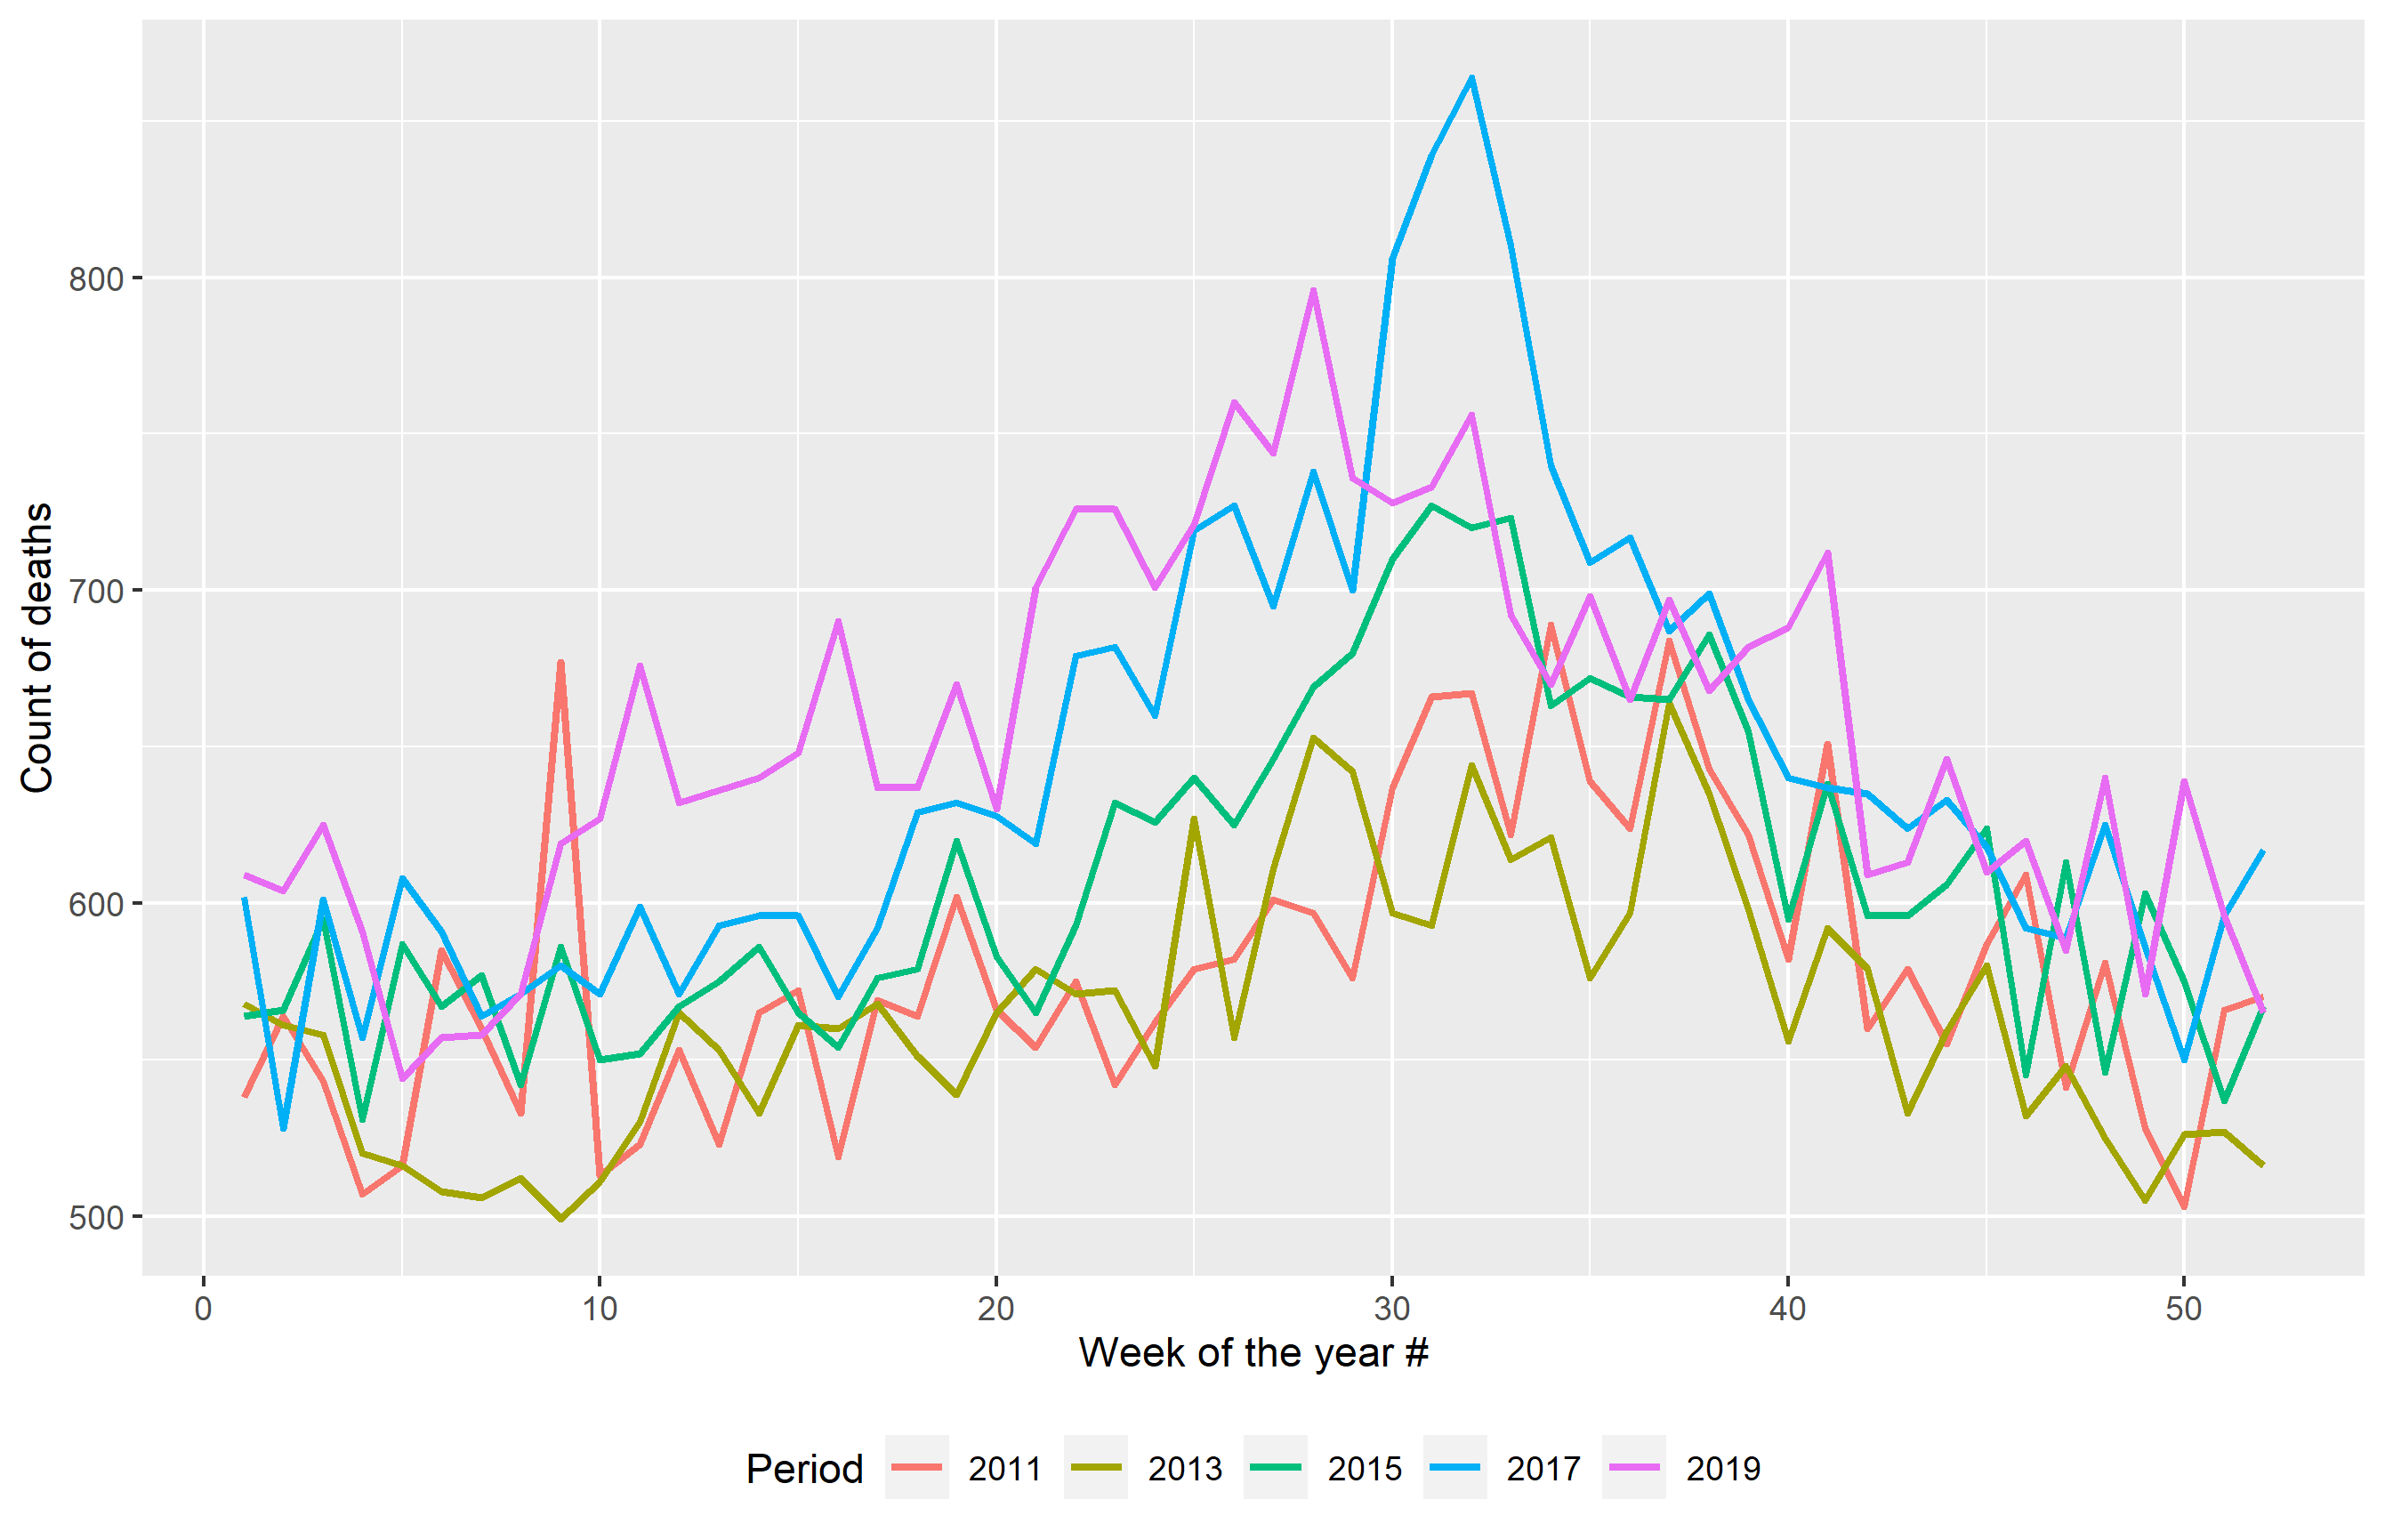
\includegraphics[width = 1.0 \columnwidth]{plots/deaths_across_years} 
caption[Weekly deaths across 2011 - 2019]{Weekly deaths across 2011 - 2019 for selected years. The peak in the middle of the year is due to increased mortality in the winter, usually driven by respiratory illnesses.} 
\label{fig:deaths_data} 
\end{figure}


\paragraph{Population data} Population data are extracted from population estimates published by Statistics New Zealand. These population estimates are produced quarterly, at a single-year-of-age breakdown, and are currently available up to the end of 2021 (Q4 2021). These population estimates are 'as at' population estimates, i.e. the population as at the end of the quarter. To estimate death rates for a given period (e.g. week), the denominator must be the population at risk over that period. This population is not closed during the period, i.e. individuals enter (e.g. through births or aging) and exit (e.g. though deaths and aging) the population of interest. Therefore, population denominators for death rates are generally measured in terms of person-time (e.g. person-years), which requires access to unit-record population data that is usually not available. 

A common approximation to this period population denominator is the mean population over the period, i.e. the mean of the populations at the start and end of the period. Since our population estimates are produced quarterly, we establish a mean weekly population by assigning to each week in the quarter the mean population for that quarter, which is the mean of the population at the start and end of the quarter. We do not make any extra adjustments for ageing effects of the population across the three months of the quarter -- the mean populations satisfactorily accounts for this since the population counts are large enough to give good approximations of the period populations. We will further discuss the derivation of the population denominators used in estimating the rates in~\nameref{subsec:death_rates}.


%-----------------------------------------------------------------
\subsection{Estimating death rates}\label{subsec:death_rates}
%-----------------------------------------------------------------

As discussed earlier in~\nameref{sec:method}, we need to understand changes in death rates for any meaningful comparison of deaths prior to and since the pandemic. To derive the age-specific death rates we take the observed death counts in each age group, at a particular time, and divide by the relevant population that is exposed to death (i.e., the population of that age group). This is described mathematically as follows:
% 
\begin{equation}
r_{(i,t)} = \frac{d_{(i,t)}}{P_{(i,t)}} \; c \;,
\label{eq:death_rate}
\end{equation}
% 
where $r_{i,t}$ denotes the death rate in age group $i$ at time $t$;, $d_{i,t}$ the death counts, and $P_{i,t}$ the population at risk. The constant $c$ is a conversion factor to convert the population units, which is generally expressed in terms of \textit{person-time} (e.g. person years). 

The crude death rates can similarly be defined by aggregating the age groups -- that is,
\begin{equation}
r_{t} = \frac{\sum\limits_{i} d_{(i,t)}}{\sum\limits_{i} P_{(i,t)}} \; c \;.
\label{eq:crude_death_rate}
\end{equation}
%
In this analysis, $t$ denotes the year and week combination, and $i$ the age group. 

\paragraph{Explanation of person-time} As described in~\nameref{subsec:data}, the population over the period of interest is not closed, and therefore, the population denominator is generally measured in terms of \textit{person-time} instead of person counts\footnote{\textit{Person-time} is the actual time a person is exposed to risk. For a given age group and a given time period, this is computed by summing how much time each person in the population lives in that period and age group.}. Typically, death rates are expressed as deaths per $100,000$ person-\textbf{years} lived, in which case, the period of interest is one year and the conversion factor is $c = 100,000$. In our case, because the period of interest is a week (i.e. we are dealing with weekly data), which implies that the unit of the population is person-weeks.

\paragraph{Population time series} As noted in ~\nameref{subsec:data}, currently population estimates are not available on a weekly basis. Therefore, for a given quarter of the year, the mean quarterly population is used across all weeks in that quarter. For example, when using equations \eqref{eq:death_rate} and \eqref{eq:crude_death_rate} to compute the death rates for the first week of 2012, the population of the first quarter of 2012 would be used, same as for the sixth week. The mean quarterly population is an approximation of the weekly period population denominators -- the aactual (unobserved) weekly population denominators may be above or below this mean.

%---------------------------------------------------------------------
\subsection{Expected deaths -- averages of pre-pandemic death rates}
\label{subsec:average_deaths}
%---------------------------------------------------------------------

A simple way to examine whether the current observations of deaths are in excess is to use the estimated death rates described in ~\nameref{subsec:death_rates} to obtain the mean death rates over the pre-pandemic years, for each age group, and compare how death rates during the pandemic years track against these pre-pandemic rates. 

For our purposes, for each age group and for each of the weeks 1 to 52, we take the mean death rate over the years 2012 to 2019\footnote{2011 is excluded due to the spike in mortality in younger age groups as a result of the Christchurch earthquakes.} and construct the "average pre-pandemic year". We present estimates of one standard deviation around the mean as an indicator of the range of death rates that one may expect under "normal" circumstances. We note that given there are only eight observations used in the calculation, the standard deviation may be relatively volatile. We provide it as a guide of the range that can exist within the data.\footnote{We have refrained from using the extreme observations for a given year in 2012 -- 2019 (For example, the year with the lowest death rate) because there is no consistently low and high death years across all age groups. For example, a year with a high winter peak may have a lower than average spring and summer death rate.}

\begin{figure}[htb!]
\centering 
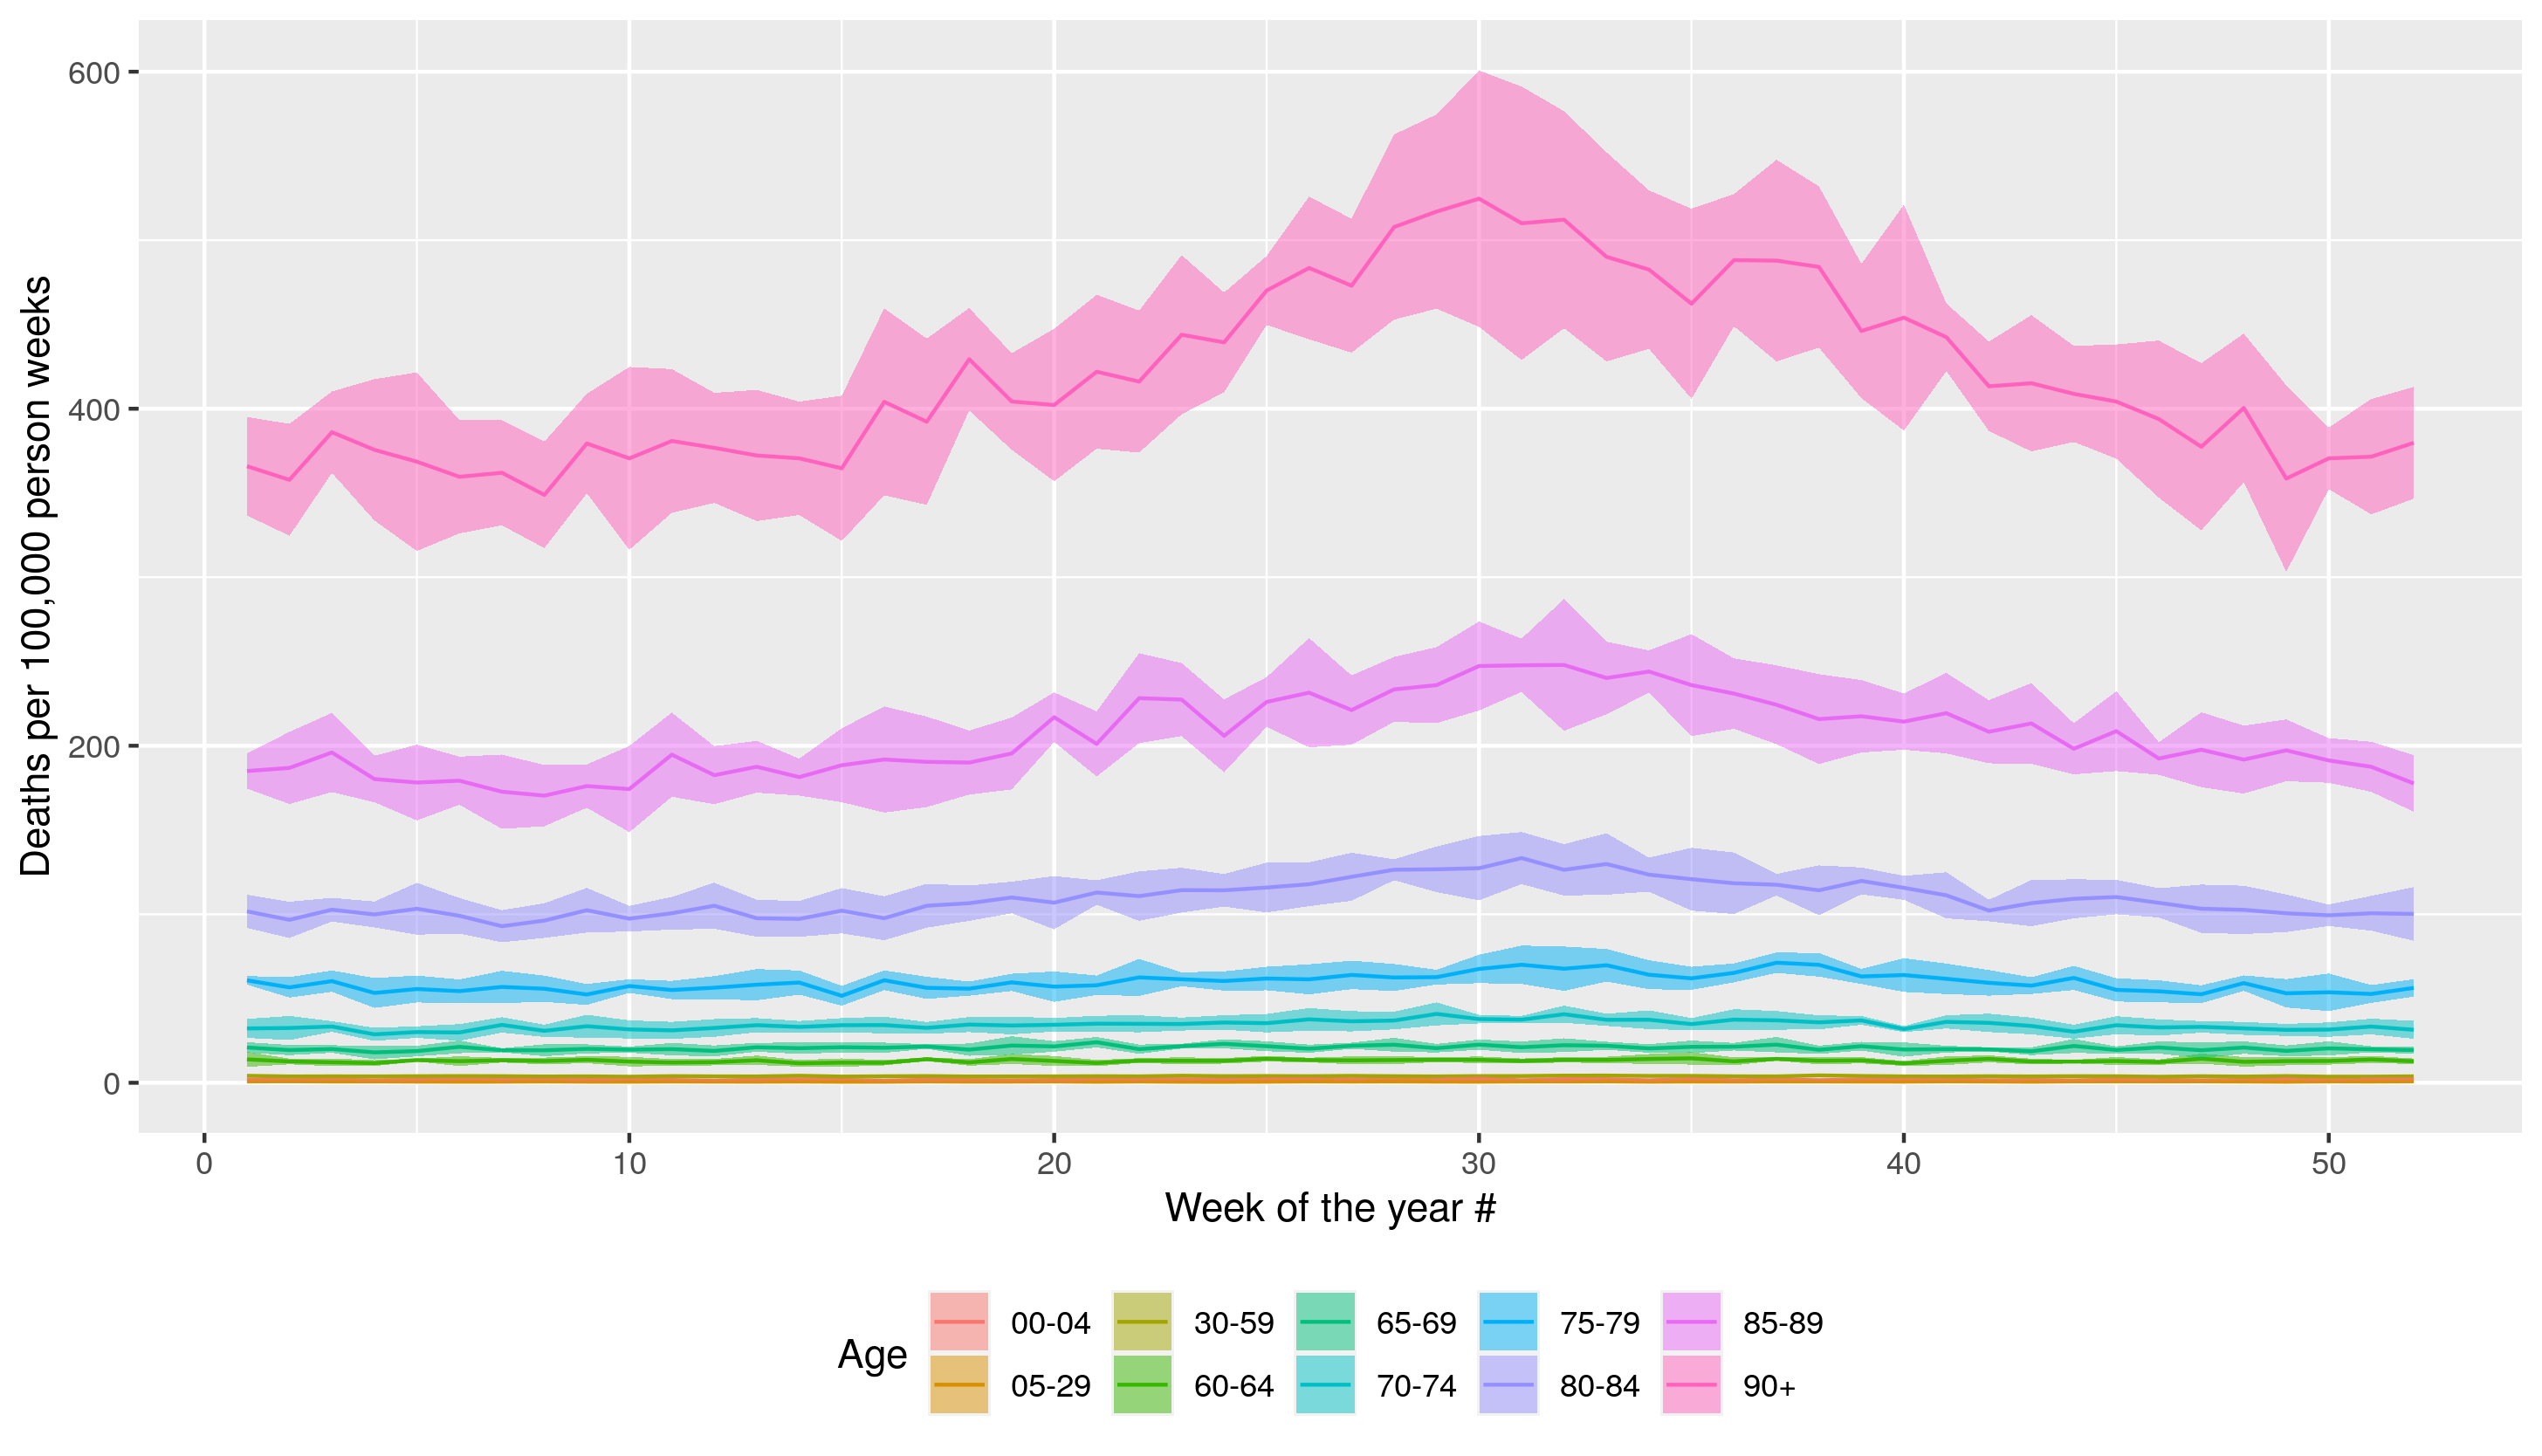
\includegraphics[width = 1.0 \columnwidth]{plots/mean_death_rates} 
\caption[Mean death rates pre-COVID]{Mean weekly death rates across 2012 to 2019, depicting what the death rates in an "average pre-pandemic year" would look like. As the age increases, we see the expected increase in death rates. As before, the peak in the middle of the year is due to increased mortality in the winter. The line represents the mean death rate, and the shaded area is $+/-$ one standard deviation about the mean.}
\label{fig:mean_death_rates} 
\end{figure}

Figure~\vref{fig:mean_death_rates} shows how these rates track across the average year. One of the major drawbacks with this method is that if the \emph{rates themselves are changing systematically over the years} examined (rather than fluctuations around a mean) -- then such changes will be obscured, and may lead to mis-identification of excess (or deficit) deaths. These issues can be addressed by using a projected deaths approach. This will be discussed in section~\vref{subsec:projected_deaths} when the methodology is released.


%---------------------------------------------------------------------
\subsection{Expected deaths -- extrapolation from pre-pandemic rates}
\label{subsec:projected_deaths}
%---------------------------------------------------------------------

Currently we are exploring methods for extrapolation of death rates -- this document will be updated once that measure has been established.


%----------------------------------------------------------------------------------------
%	RESULTS AND DISCUSSION
%----------------------------------------------------------------------------------------

%--------------------------------------------------
\section{Observed deaths vs. expectations}
%--------------------------------------------------

After establishing a measure of expected deaths as discussed in section ~\vref{subsec:average_deaths}, we compare the observed rates through the three pandemic years (2020, 2021, and 2022 so far) to the expected rates. While the interpretations around variability can be subjective, we draw particular attention to situations where the death rates are outside one standard deviation from the mean death rate observed in pre-pandemic years, especially if that maintains over a period of weeks.

\begin{figure}[tb]
\centering 
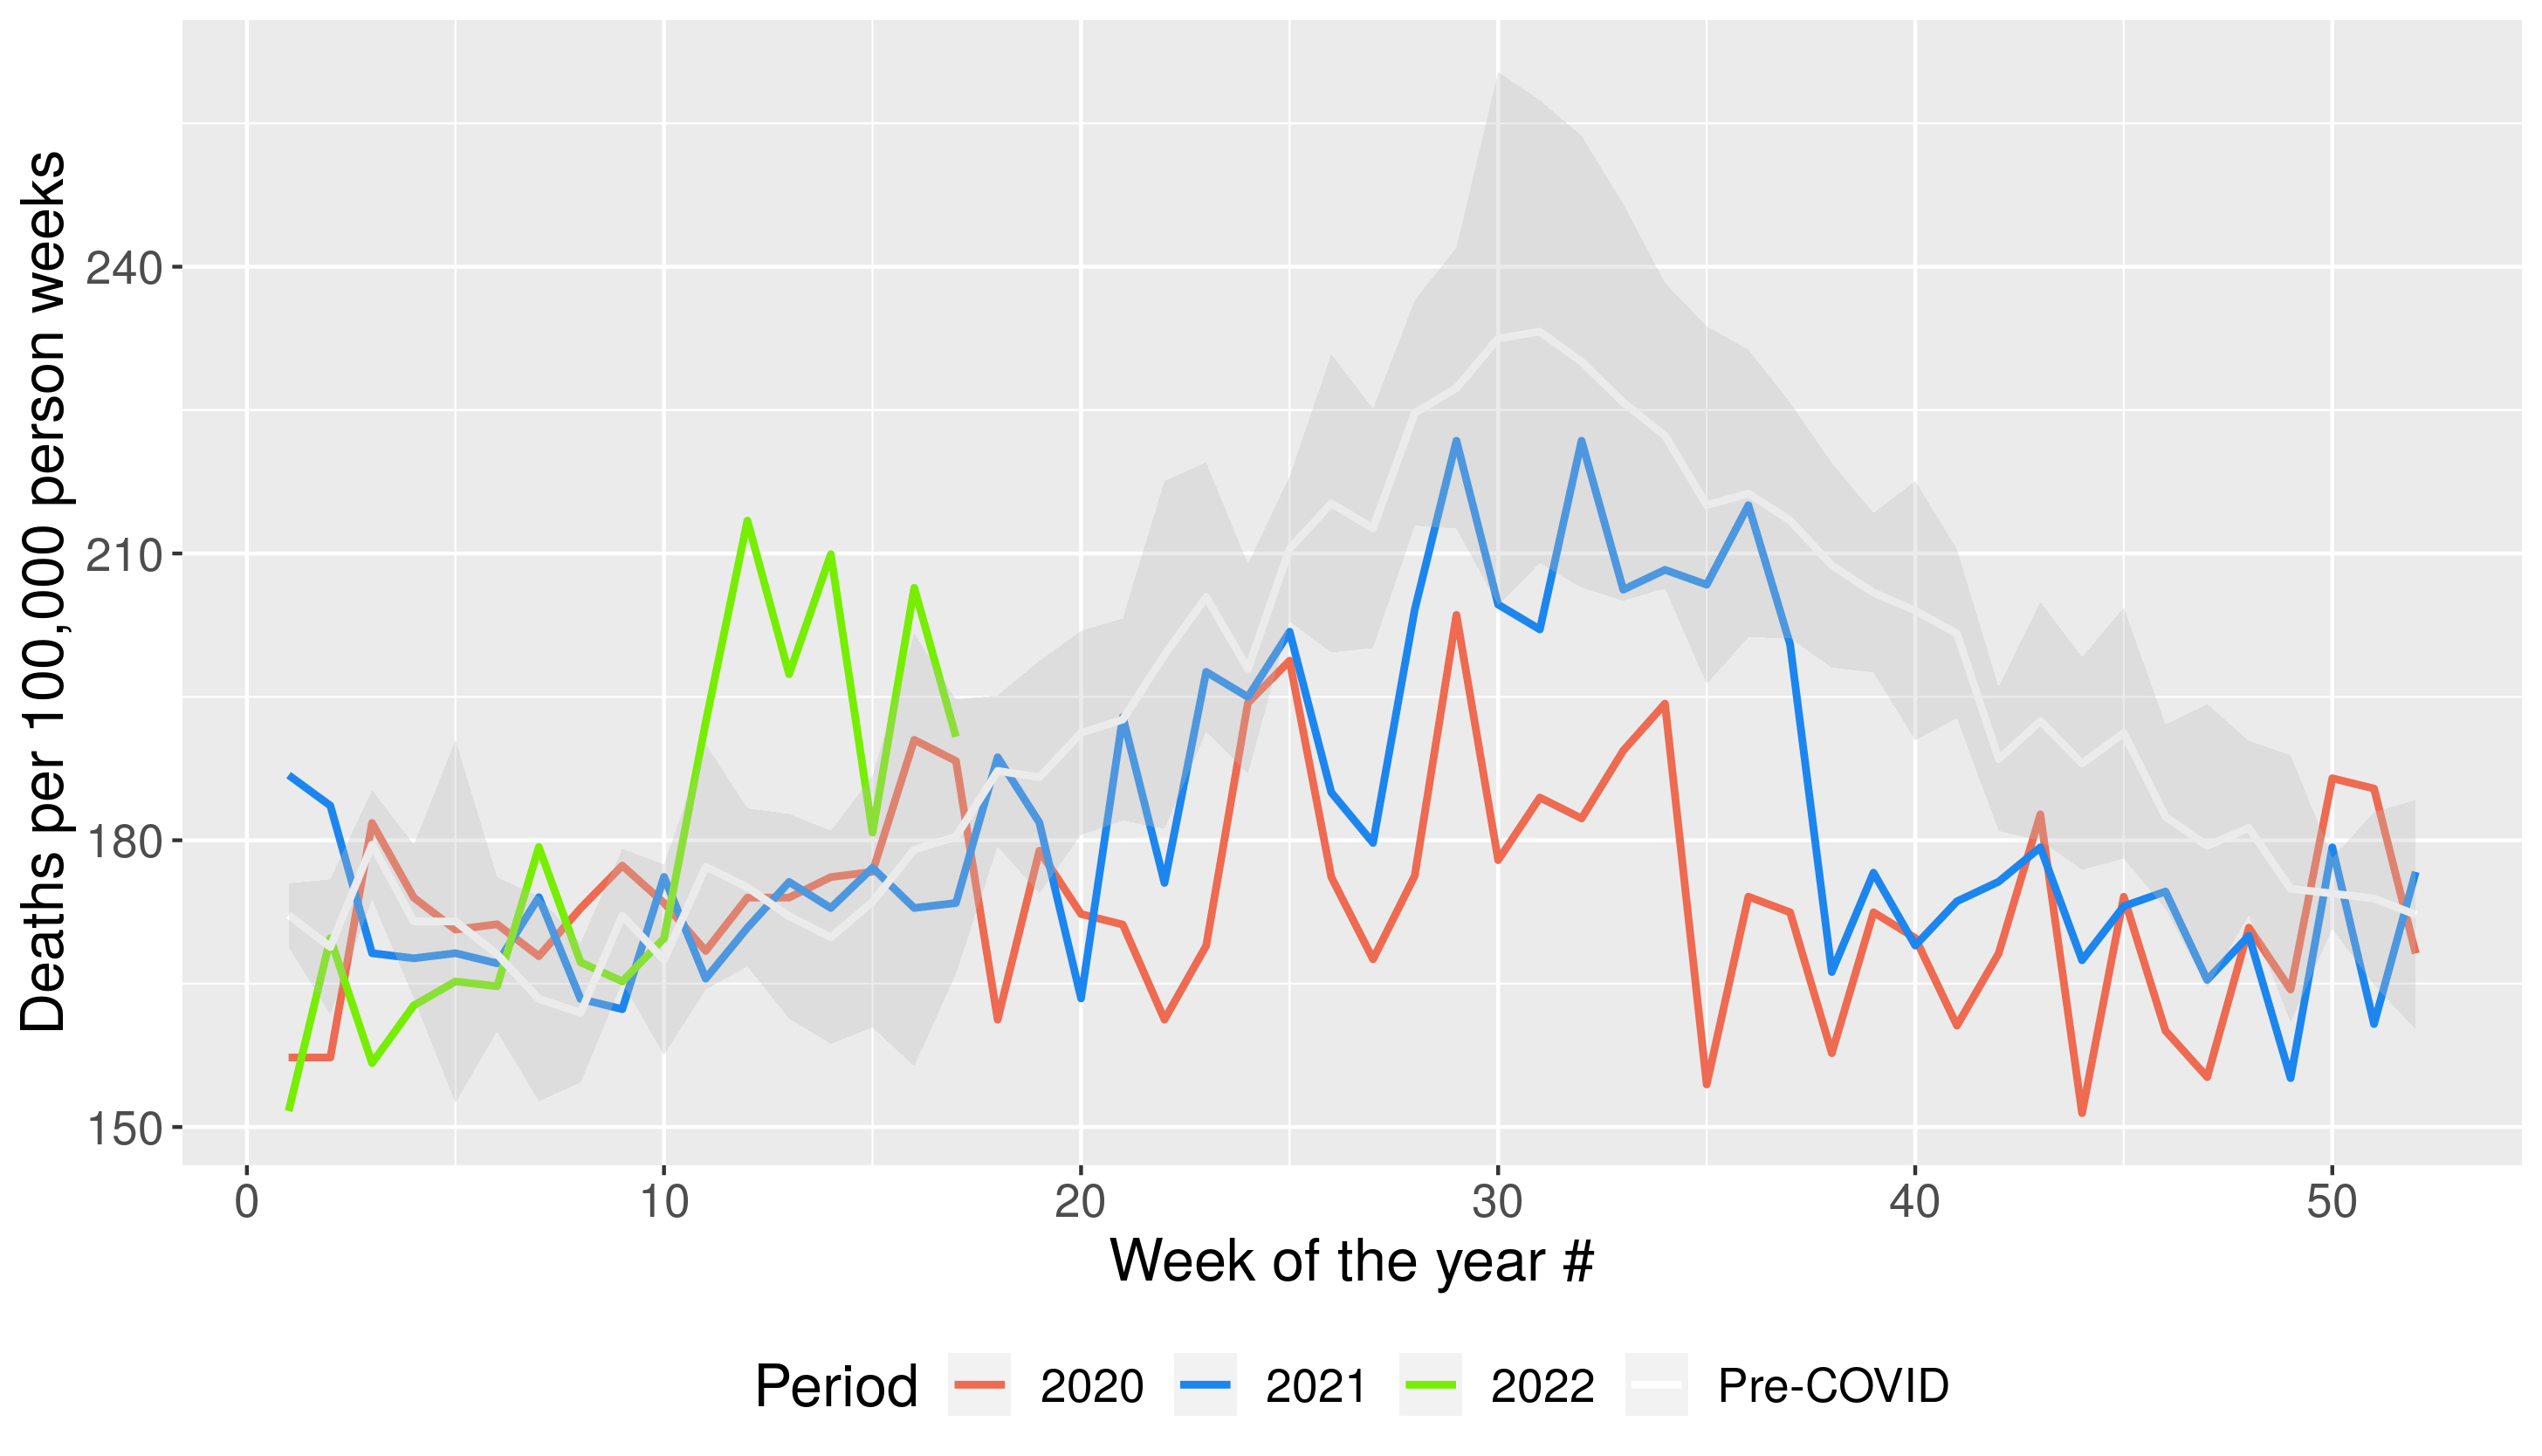
\includegraphics[width=1.0\columnwidth]{plots/deaths_over_80} 
\caption[Death rates in the over 80 age group]{Comparison of death rates for the \textbf{80+} age group. We can see that in 2020 the death rates were lower than typical, while 2021 sees them beginning to approach typical patterns.}
\label{fig:over80_rates} 
\end{figure}

Figure~\vref{fig:over80_rates} shows the comparisons across the three pandemic years. Notably in the older ages, 2022 death rates are tracking higher than expected. In other age groups, we do not yet see much of a signal in terms of "excess deaths" in 2022. 

It should be noted that since we are observing all-cause mortality, if other drivers caused more deaths than is "typical" (e.g., respiratory syncytial virus, influenza, etc.), this would also be observable in this measure. Because we do not have robust cause of death data at the timeliness required, these specific drivers cannot be examined or separated.


%----------------------------------------------------------------------------------------
%	BIBLIOGRAPHY
%----------------------------------------------------------------------------------------

\renewcommand{\refname}{\spacedlowsmallcaps{References}} % For modifying the bibliography heading

\bibliographystyle{unsrt}

\bibliography{measuring_deaths_refs.bib} % The file containing the bibliography

%----------------------------------------------------------------------------------------

\end{document}
